\documentclass[twocolumn,twocolappendix]{aastex631}

\usepackage{amsmath}

\newcommand{\parens}[1]{\left(#1\right)}
\newcommand{\brackets}[1]{\left[#1\right]}

\begin{document}
\author{Jack T. Dinsmore}
\affiliation{Stanford University, Department of Physics}
\title{Compton Scattering of Accretion Disk Emission off Black Hole Coronas in Curved Spacetime}

\begin{abstract}
  Raytraced images of black hole event horizons, accretion disks, and coronas are presented for the Schwarzschild and Kerr metrics. The physical parameters of the system are adjusted to gain a qualitative understanding of the physics at play in the strong lensing, compact object system.
\end{abstract}

\section{Introduction}

General Relativity (GR) bends the trajectories of light in the presence of strong gravity. Weak examples of this effect have been observed in the context of gravitational lensing \citep{blandford1992cosmological}, which is a useful technique in cosmology. But near compact objects such as black holes (BH), light is bent so strongly it may curve into a circular orbit or be consumed by the BH's event horizon (EH). Here, computationally intensive methods such as ray-tracing must be employed to model the lensing effect.

Ray tracing is the act of numerically integrating the equation of motion of a photon along its path to model radiative dynamics \citep{vincent2011gyoto}. The technique is employed in many scenarios. One example is the imaging of accretion disks, which has been simulated as far back as in the 70s \citep{luminet1979image} and in 2019 observed by the Event Horizon Telescope (EHT) \citep{collaboration2019first}. But even when the accretion disk is not resolved, strong lensing is still a crucial effect. Examples include BH spectra \citep{cunningham1975effects}, the polarization of BHs \citep{dovvciak2008thermal} and electromagnetic signatures from BH mergers \citep{d2018electromagnetic}.

A benefit of ray tracing is that it allows the accurate modeling of complicated radiative features of a BH, such as an accretion disk and a corona. An accretion disk is a large disk of cool matter accelerating into the BH, fed by nearby stars or other matter sources, and radiating thermally. The total radiation of this disk is bounded above by the Eddington luminosity, beyond which the radiation pressure produced by accretion would prevent more matter from falling into the BH, thereby ending the process.

A BH corona represents matter which has freely fallen from far away into the black hole, and has therefore picked up kinetic energy on the order of its mass energy. This matter is very hot, and if it thermally interacts with other in-falling matter it becomes ionized, and the stripped electrons can equilibrate and become relativistic. Such electrons are highly apt to Inverse-Compton (IC) scatter, a process which boosts photons from the disk into higher energy bands such as X-rays or $\gamma$-rays.

In this project, we construct a simplified supermassive BH system consisting of a cool accretion disk and a hot corona. Images of the EH and its surroundings are created in the optical band and the X-ray band as various components of the system are modeled. This gives a qualitative understanding of the effect of model components such as strong lensing, accretion disk optical depth, and IC scattering.

\section{Methods}

Our simplified model for a BH depends only on the BH mass $M$, disk absorption coefficient $\alpha$, corona scale density $\rho_0$, the corona $\gamma$ factor, the BH spin $a$, and the cosmological redshift $z$. Later, we will manually choose these parameters for the sake of making an interesting picture, but in this section we will take them as fixed and derive a simplified model for the dynamics of light.

\subsection{BH Environment}

The only modeled radiative components in this simplified BH system are accretion disk emission and IC scattering in the corona. Jets were not modeled, nor distant sources of radiation such as stars or reflecting clouds. 

\paragraph{Accretion Disk} The BH itself is assumed to accrete at the Eddington limit, generating luminosity 
\begin{equation}
  L_\text{tot} = \frac{4\pi GMm_pc}{\sigma_T}
\end{equation}
where $m_p$ is the mass of the proton and $\sigma_T$ is the Thomson cross section.
We model this luminosity as emitted near the BH and absorbed and re-emitted as black body radiation by the surrounding gas. Since the cross-sectional area of this disk increases with radius $r$, its flux obeys
\begin{equation}
  \begin{split}
    F(r) &= \frac{L_\text{tot}}{4\pi r^2} \\&= \parens{1.14\times10^{26}\frac{\text{erg}}{\text{s\ cm}^2}}\parens{\frac{M}{M_\odot}}^{-1}\parens{\frac{r}{r_S}}^{-2}.
  \end{split}
\end{equation}
and its temperature decreases as $F = \sigma T^4$ where $\sigma$ is the Stefan-Boltzmann constant, or
\begin{equation}
    kT(r) =(3.2\ \text{keV})\parens{\frac{M}{M_\odot}}^{-1/4}\parens{\frac{r}{r_S}}^{-1/2}.
    \label{eqn:disk-temp}
\end{equation}
This temperature may redshifted by doppler boosting, gravitational redshift, or cosmological redshift $z$.

Far enough from the BH, this disk flares due to the reduced BH gravity forcing the disk to collapse into a plane; assuming an ideal gas, the vertical density profile of this structure is Gaussian, with scale height
\begin{equation}
  H(r) = (3.7 \times 10^{-3} r_S) \parens{\frac{M}{M_\odot}}^{-1/8}\parens{\frac{r}{r_S}}^{5/4}.
\end{equation}
Precisely, this scale height is the standard deviation of the Gaussian. The disk is spatially quite thin; even at $10 r_S$ from the BH, the disk is only a few percent of a Schwarzschild radius thick. For the sake of collisions, we therefore model the disk as two-dimensional, with optical depth
\begin{equation}
  \tau(r) = \frac{\sqrt{2\pi}\alpha H(r)}{\hat{\mathbf z} \cdot \hat{\mathbf v}}.
\end{equation}
for absorption coefficient $\alpha$. Unit vectors $\hat{\mathbf z}$ and $\hat{\mathbf v}$ are the normal vector of the accretion disk and the light velocity respectively. We assume $\alpha$ is wavelength- and temperature-independent in the optical band.

We model the velocity of the disk as Keplerian, with velocity distribution
\begin{equation}
  \beta(r) = \sqrt{\frac{r_s}{2r}}
\end{equation}
so that doppler shift will be visible. This formula is invalid for $r < 2 r_s$, so there will in principal be a cutoff for small radii. But this matter will be so doppler boosted that it will not be in the visible band and therefore not relevant here.

\paragraph{Corona} The corona's formation mechanism implies that each constituent particle is at approximately escape velocity, with Lorentz factor $\gamma \approx 1 + (r_S/r)^2/2$ at altitude $r$ above the singularity. Since $r > r_S$, this is only mildly relativistic. We assume that these particles collide and thermally equilibrate near the BH, in which case the proton $\gamma_p$ factor remains mostly unchanged and the electron $\gamma_e$ factor is boosted to $(\gamma_e -1) = (\gamma_p - 1) (m_p / m_e)$, so that both particles have the same kinetic energy. These $\gamma$ factors are assumed to be constant throughout the corona. Appendix \ref{app:corona-density} derives the following density distribution of particles under the assumption of hydrostatic equilibrium:
\begin{equation}
  \begin{split}
  \rho(r) = \rho_0 &\left[1 + \parens{\frac{9}{4(\gamma_p-1)}}\parens{\frac{r_S}{r}}\right.\\
  &+ \left. \frac{1}{2}\parens{\frac{9}{4(\gamma_p-1)}}^2\parens{\frac{r_S}{r}}^2\right],
  \end{split}
\end{equation}
where $\rho_0$ represents some scale density.

The boosted electrons IC scatter accretion-disk photons of energy $\mathcal{O}(\text{keV})$ by equation \ref{eqn:disk-temp} to high-energies with cross section $\sigma_C\approx \sigma_T$, since the photon energy is so low compared to the electron mass energy of 511 keV. This means that the probability of a scatter for a photon ray crossing distance $dr = r_S d\ell$ is
\begin{equation}
  \frac{dp}{d\ell} = \frac{r_S \sigma_T}{m_e} \rho(r) = \parens{2.16 \times 10^8\ \frac{\text{cm}^3}{\text{g}}}\parens{\frac{M}{M_\odot}}\rho(r)
\end{equation}
The process of IC scattering boosts the photon energy by a factor of $\sim\gamma_e^2$. Since $\gamma_e^2 \gtrsim 511$, the boosted photon will have energy greater than to the rest-mass energy of the electron and $\sigma_C$ will be sharply decreased. For this reason, we  assume that each photon is IC-scattered only once.

IC-scattered photons are ejected roughly parallel to the initial electron velocity in this highly relativistic case, so the angular distribution of IC-scattering is the angular distribution of corona electron velocity. We assume for now that this distribution is isotropic.



\subsection{Relativistic Ray-Tracing}

Since BH physics is set in strongly curved spacetime, all radiative processes must take GR into account. We do this by back-propagating the path each light ray takes from the observer to its source. We perform this propagation with a static metric (either Minkowski, Schwarzschild, or Kerr), which defines the metric tensor $g_{\mu \nu}$ and Christoffel symbols $\Gamma_{\mu\nu}^\lambda$. The metric and symbols are derived in Ref.~\cite{muller2009catalogue}.

The geodesic equation gives that, for a light ray of velocity $u^\mu$,
\begin{equation}
  \frac{d}{d\lambda}u^\mu = -\Gamma^\mu_{\rho \sigma}u^\rho u^\sigma.
  \label{eqn:accel}
\end{equation}
where $\lambda$ is some parameterization of the light's trajectory, obeying 
\begin{equation}
  \frac{d}{d\lambda}x^\mu = u^\mu.
  \label{eqn:vel}
\end{equation}
Eqs.~\ref{eqn:accel} and \ref{eqn:vel} form a coupled system which are numerically integrated with finite step size $d\lambda$. Because we back-propagate the light, $d\lambda < 0$. 

To reduce numerical inaccuracy, every few iterations, the light velocity is adjusted to ensure it is null:
\begin{equation}
  u^\mu u_\mu = u^\mu u^\nu g_{\mu\nu} = 0.
\end{equation}
It is also key to reduce the step size of $d\lambda$ when near a coordinate singularity, such as an EH or the the spin axis of Kerr. Near an EH, light is infinitely redshifted meaning that $x_0 \rightarrow -\infty$. This can only be achieved if the derivatives of Eq.~\ref{eqn:accel} blow up, so in practice we stop propagating photons too close to the EH to avoid numerical error.

The only other gravitational effect we model is redshift. Gravitational redshift for a photon produced at a point in spacetime with metric $g_{\mu\nu}$ is  $1 + z = \sqrt{g_{00}}$, assuming that the observer is at infinity where $g_{00} = 1$. Doppler redshift is also included for matter moving relative to the observer.

When a light ray encounters the accretion disk at radial coordinate $r$, we assume that some fraction $1-e^{-\tau(r)}$ of the light was radiated there. We then propagate the remaining $e^{-\tau(r)}$ until it becomes negligibly small or escapes the BH. When an IC event occurs, we scatter the light ray in a uniformly random direction. Due to this random scattering, we must re-propagate the middle-most light rays multiple times avoid small-sample noise. This presents the primary barrier from a computational perspective.


\section{Results \& Discussion}
The BH properties we use are displayed in table \ref{tab:props}. The BH mass was chosen to be that of Messier 87, and the corona proton $\gamma$ was chosen to be the value from class, which also corresponds to the energy a proton gains by falling from infinity to radius $r = r_S$. The other parameters were chosen for the sake of making appealing images. A large redshift was chosen to shift accretion disk temperatures into the visible range, and a large spin was chosen to maximize the difference between the Kerr and Schwarzschild metrics. The absorption coefficient corresponds to an average optical depth of $\tau = 1$ at the innermost stable circular orbit (ISCO), and greater towards the edge of the image.

The observer is placed $10r_s$ away from the BH singularity, slightly above the disk, where gravitational effects are small. A single image consists of 150,000 rays of light. For images that also include IC scattering, the numerical integration requires many photons to be run multiple times, resulting in about 9 million simulated photons per image.

\begin{table}[htbp!]
  \centering
  \begin{tabular}{cc}
    \hline \hline 
    Property  & Value \\ \hline
    Mass ($M$) & $2.4 \times 10^{12} M_\odot$ \\ 
    Absorption coefficient ($\alpha$) & $500/r_S\ (1.7\times 10^{-3}$ cm$^{-1}$) \\ 
    Corona scale density ($\rho_0$) & $5 \times 10^{-26}\ \frac{\text{g}}{\text{cm}^3}$ \\ 
    Proton Lorentz factor ($\gamma_p$) & $1.1$ \\ 
    Spin ($a$) & 0 or 0.8 \\ 
    Cosmological redshift ($z$) & 3.5 \\ 
    \hline \hline
  \end{tabular}
  \caption{BH properties used for this paper. $M$ was set to the mass of Messier 87, and $\gamma_p$ was set to the value given in class. The other parameters are chosen to maximize visibility of the effects at play.}
  \label{tab:props}
\end{table}

\begin{figure}[htbp!]
  \centering
  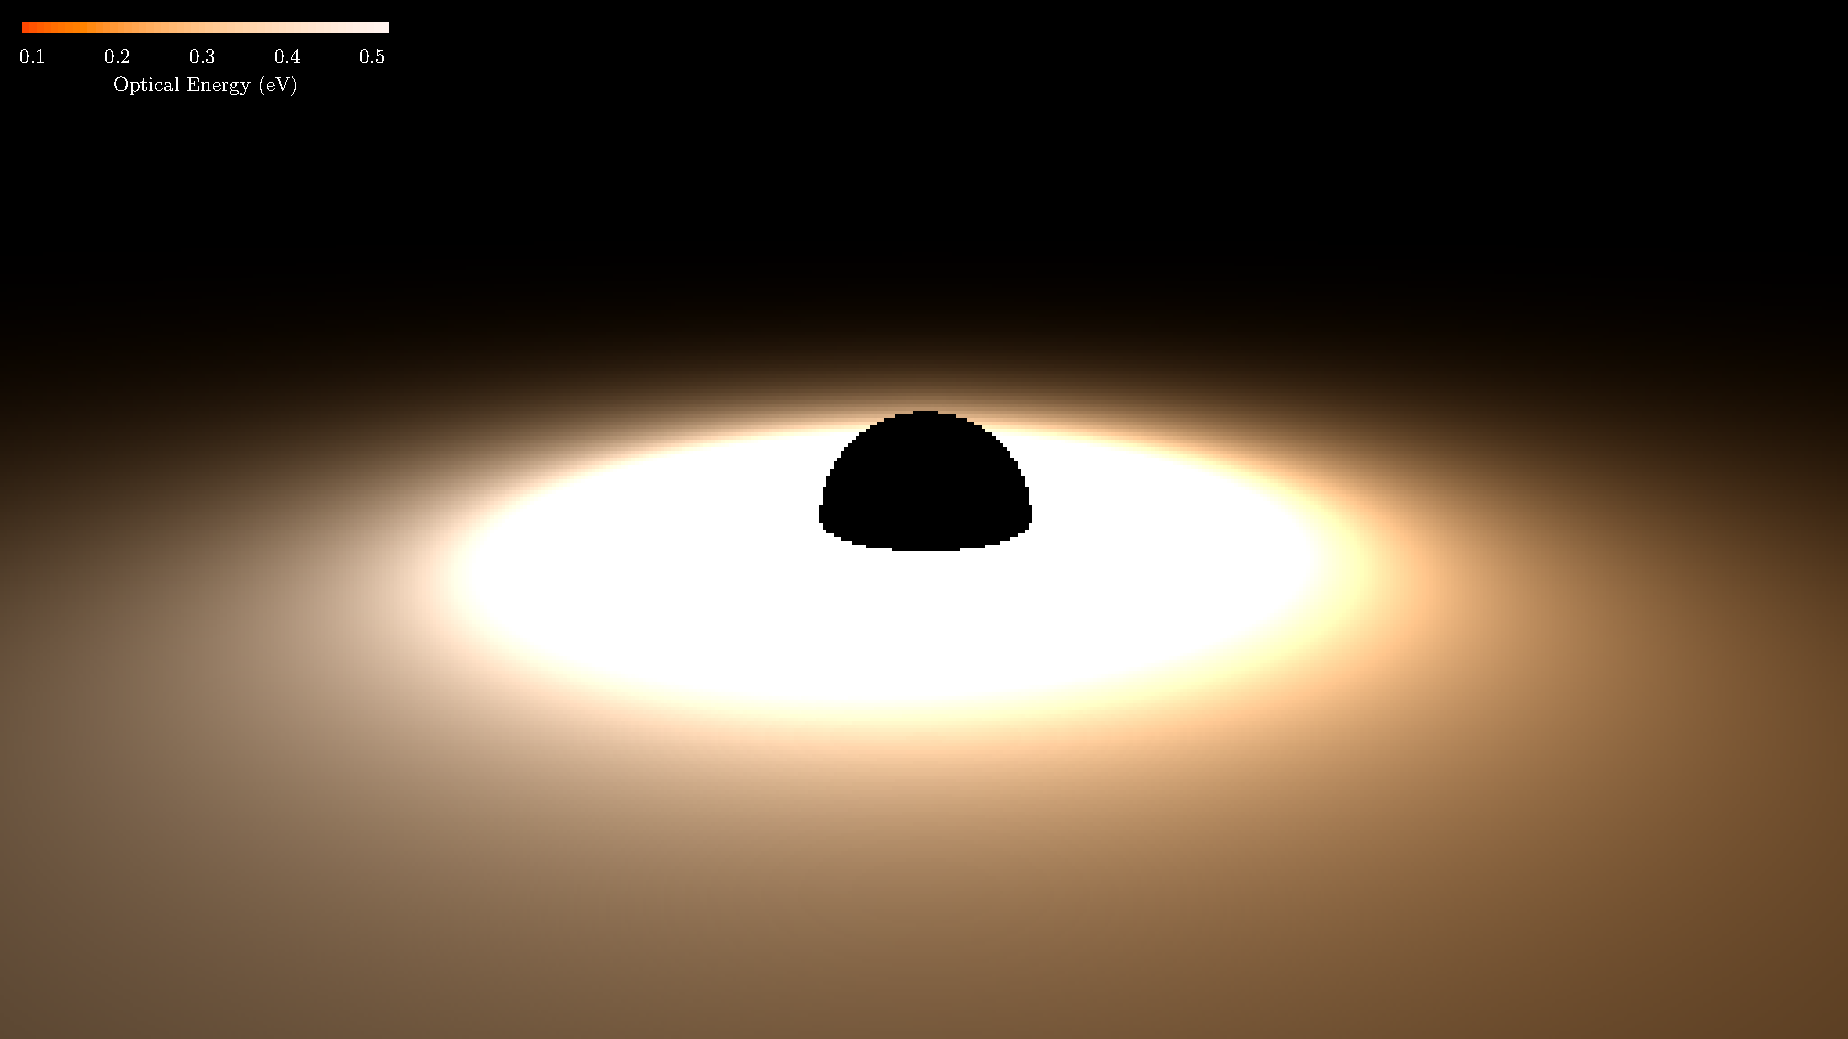
\includegraphics[width=\linewidth]{../data/minkowski-optical.pdf}
  \caption{The accretion disk rendered in Minkowski (flat) space with an opaque ball of the same width as the BH that will be added later. The black circle on the left represents the disk moving so fast that it is blue shifted out of the visible band.}
  \label{fig:mink}
\end{figure}

Below, each of the BH model components are presented in turn and analyzed in increasing order of complexity. We start with the accretion disk, adding spacetime curvature and studying the effect of accretion depth translucency. Then we consider Compton scattering, and finally we consider the Kerr metric. Throughout, the position of the observer will remain fixed. The image brightness is set for each image so that 90\% of the pixels are not saturated, except when otherwise indicated.

Figure \ref{fig:mink} displays the accretion disk presented in the flat Minkowski metric. The image is mostly for comparison, though it does show several key features of the disk, such as its luminosity and temperature dependence on radius and the the Doppler redshift of the accretion disk due to its angular velocity. This doppler shift is faint, because large $\beta$ only occurs for small $r$, and that region is so bright it appears as white in the image. A black ball with radius $1 r_S$ has been placed in the center with no lensing to depict how small the Schwarzschild radius is compared to the images that will follow. No corona is present in this image.

\begin{figure}[htbp!]
  \centering
  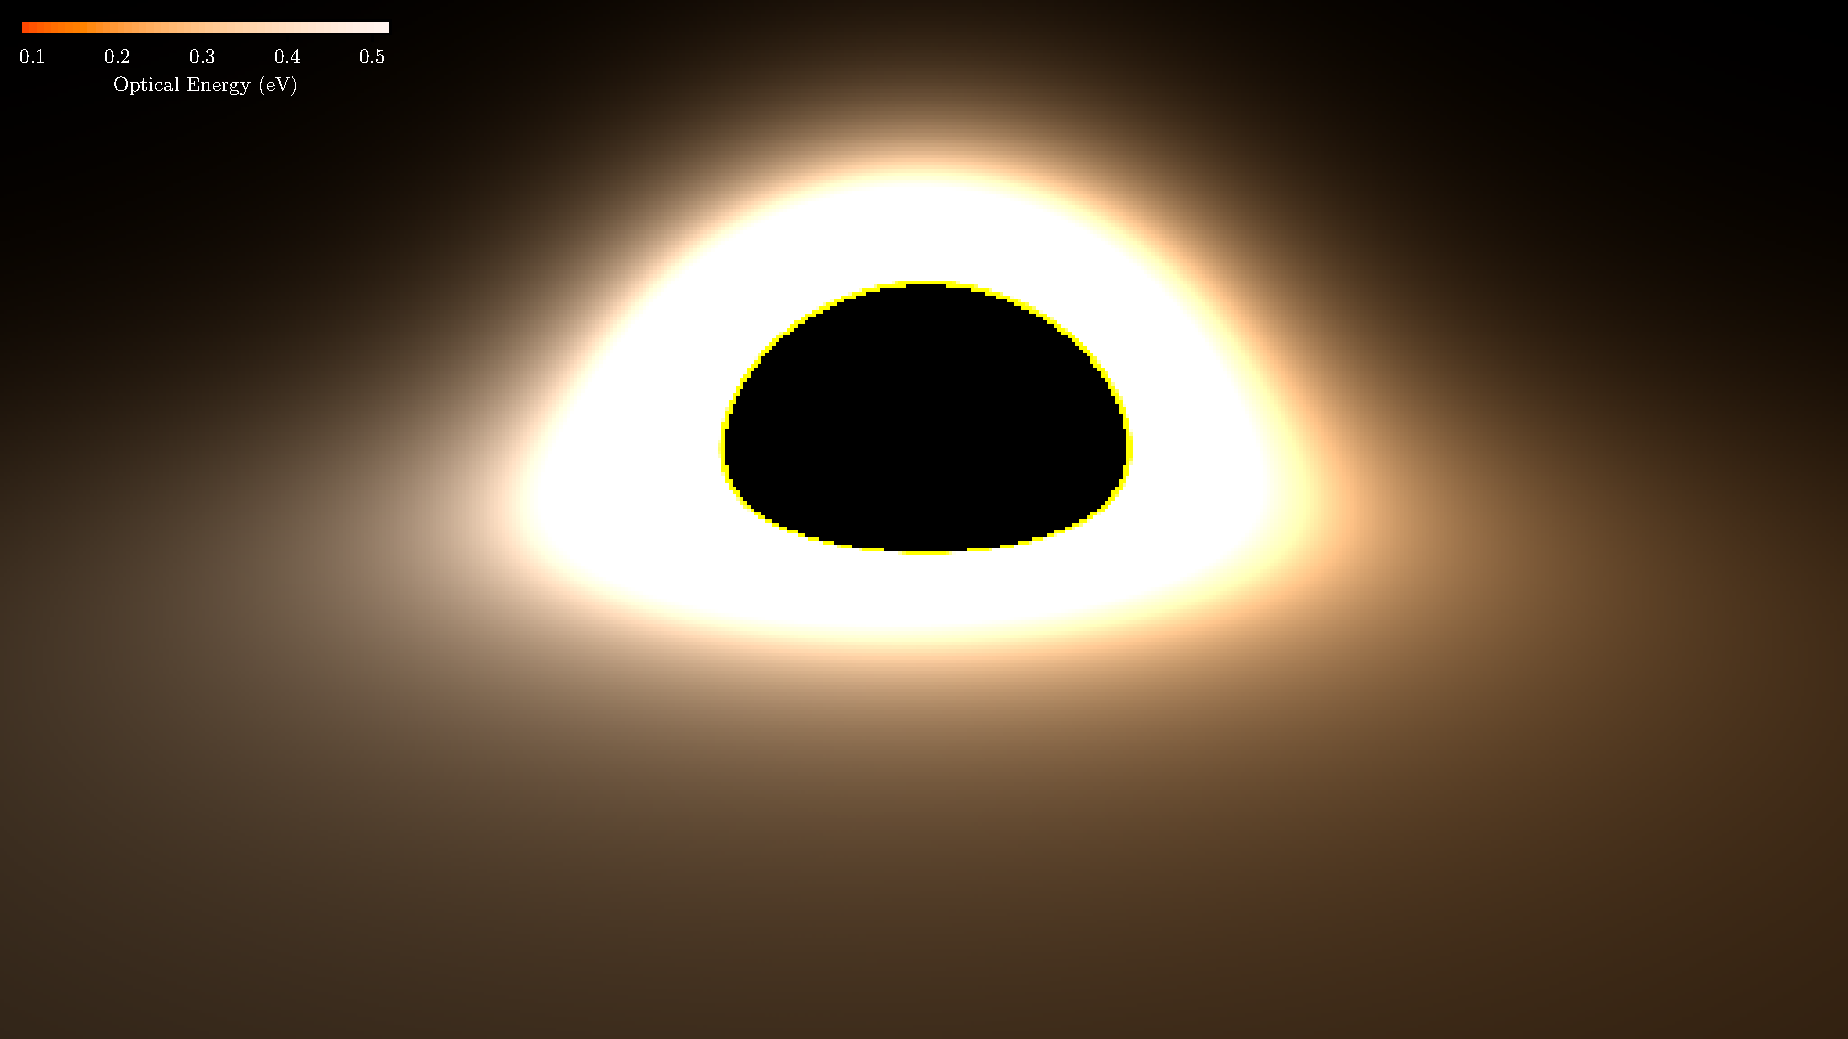
\includegraphics[width=\linewidth]{../data/thick-optical.pdf}
  \caption{The Schwarzschild spacetime with an optically thick ($\tau \gg 1)$ accretion disk. The back of the disk is lensed over the BH and appears higher in the image.}
  \label{fig:thick}
\end{figure}

\begin{figure}[htbp!]
  \centering
  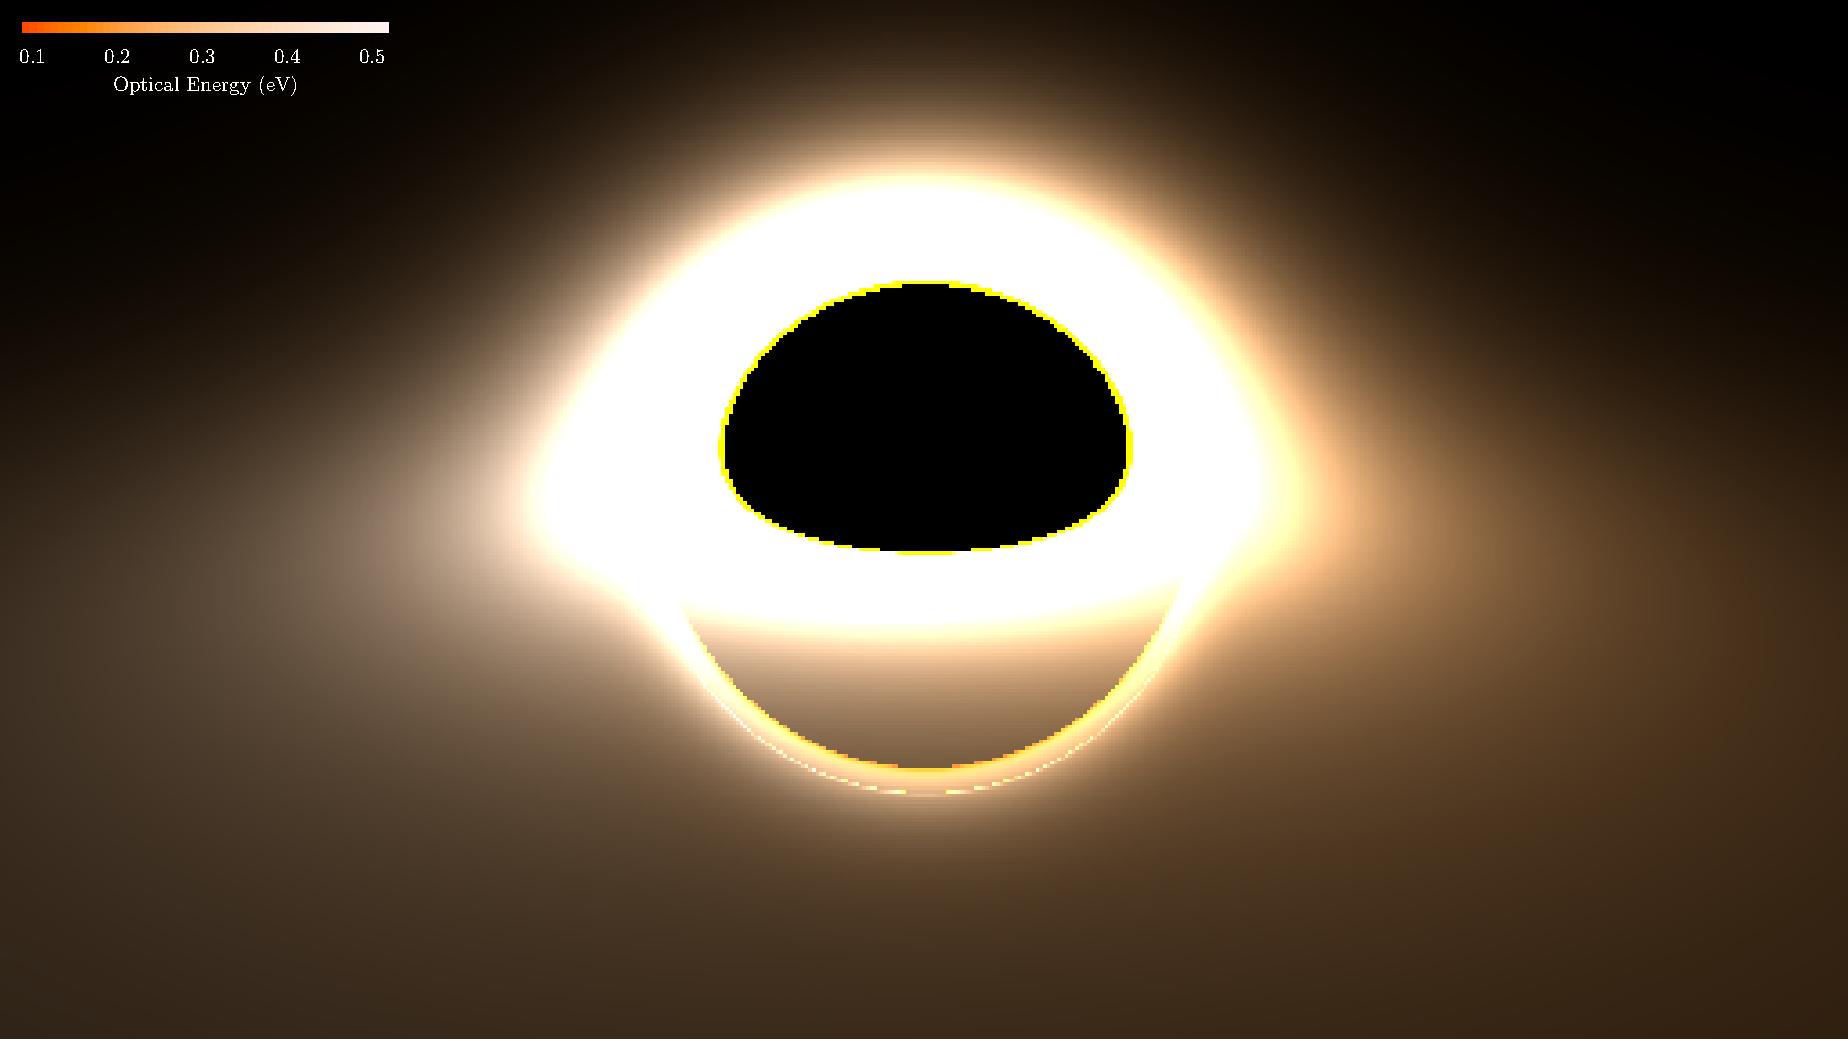
\includegraphics[width=\linewidth]{../data/thin-optical.pdf}
  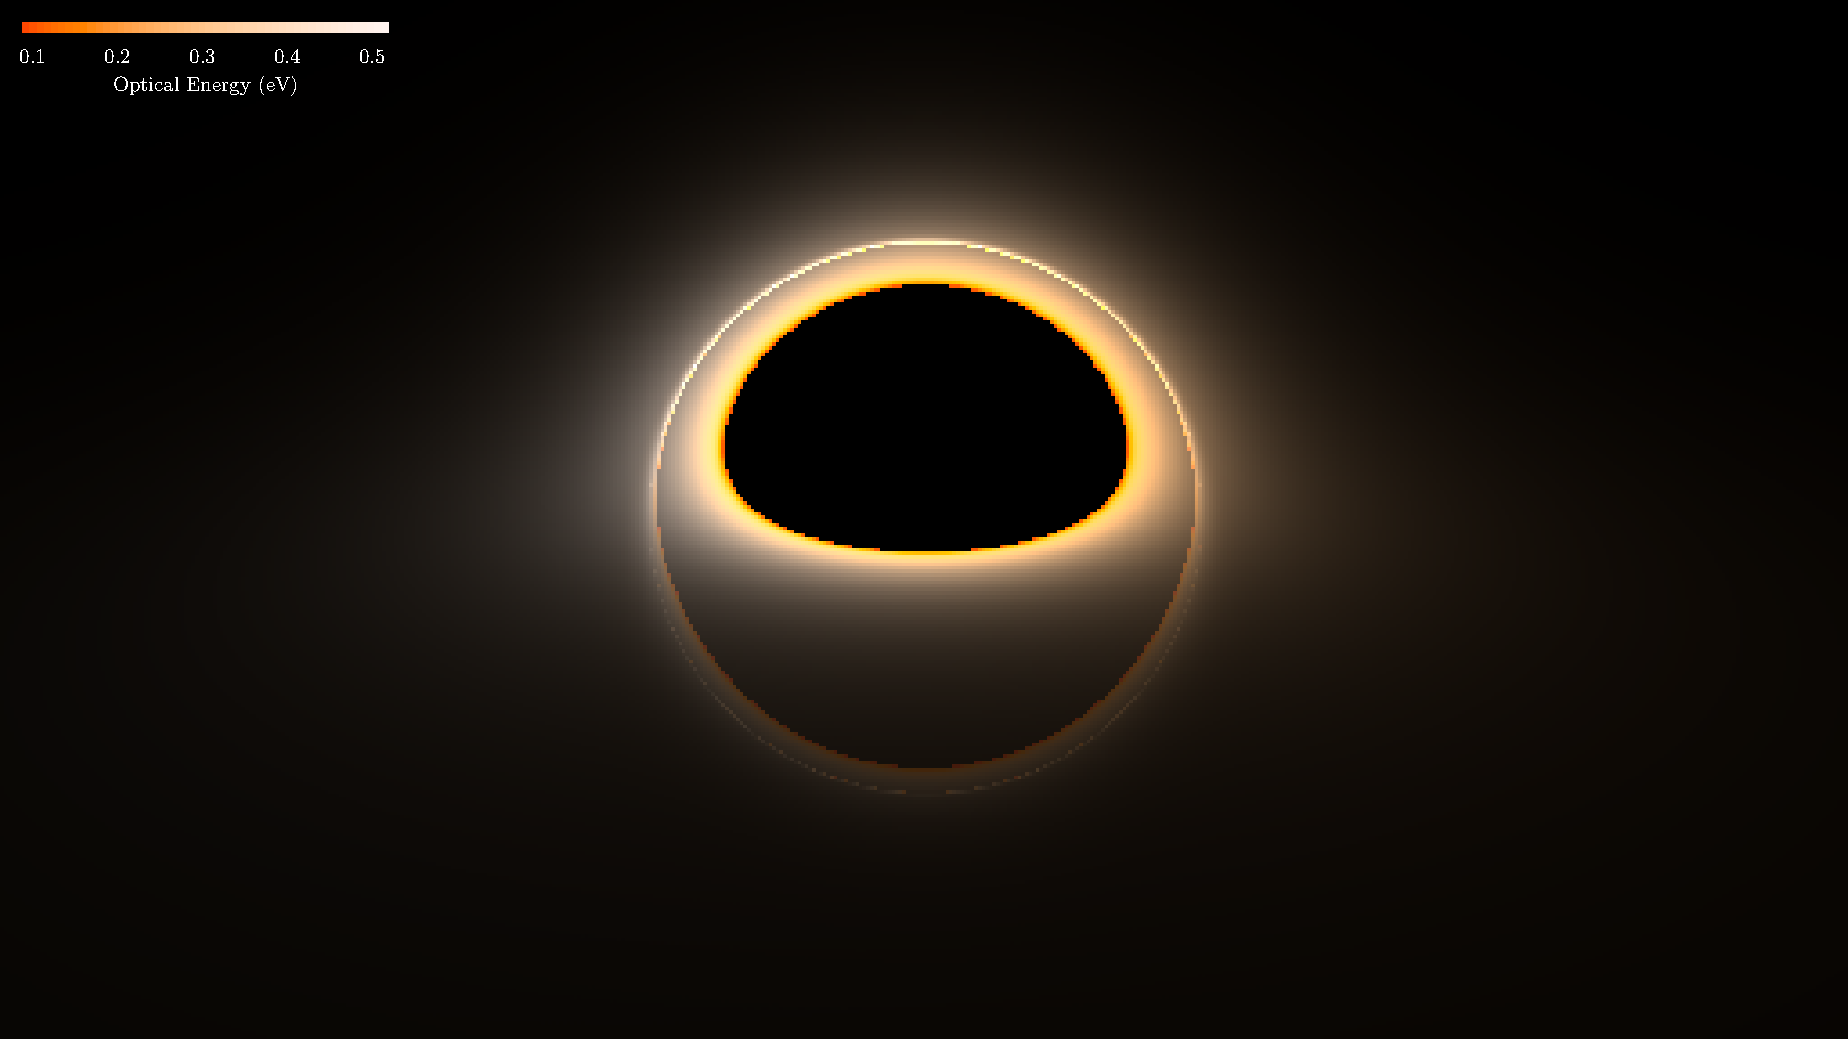
\includegraphics[width=\linewidth]{../data/thin-bright-optical.pdf}
  \caption{(\textit{Top}) The Schwarzschild spacetime with a thinner ($\tau \gtrsim$) accretion disk. The BH is observable underneath the disk, and the area around the BH is brighter. (\textit{Bottom}) The same image with contrast increased so that the photon ring is visible around the BH and gravitational redshift is visible at the edges of the BH. The rest of the accretion disk is drowned out by the bright photon ring.}
  \label{fig:thin}
\end{figure}

Figure \ref{fig:thick} shows the Schwarzschild metric added onto the accretion disk depicted in figure \ref{fig:mink}. The absorption coefficient of the disk has been raised to $\tau \gg 1$ throughout the disk and there is still no corona. All features of this image are therefore only the effect of lensing.

The disk has been visually deformed, appearing to rise above the BH where the BH is lensing light downwards towards the disk. This part of the disk is therefore brighter than it otherwise would be and has a larger effect on the overall observed properties of the BH, e.g. polarization or spectrum. The light near the BH is also brighter than for Minkowski space, making the rest of the disk look dimmer by comparison. This is another effect of lensing.

Figure \ref{fig:thin} represents the BH system with an accretion disk of the listed $\alpha$, which gives $\alpha = 1$ at the ISCO. Since some photons are allowed to pass through the disk, the EH of the BH is visible below the disk as well as above it. Just outside the bottom EH is a thin halo where light has been bent around the BH and intersects the accretion disk on the other side. This light has impacted the accretion disk twice, and therefore contains additional flux. However, since $\tau = 1$, the farther side of the accretion disk is screened by a factor of $e^{-\tau}$ and the luminosity of this region is not great. If $\tau$ were lowered, this lower half of the halo would grow brighter rapidly until it overwhelmed the upper half.

Interestingly, the upper-half and lower-half of the halo both display the same part of the disk. If a brief event occurred in that region of the disk, the effect would be visible in flux from the BH at slightly offset times, due to the longer travel time of the lower-half of the halo and the time it takes to pass through the disk. This can affect the light curve of the event, even if the BH EH cannot be resolved.

The bottom panel of figure \ref{fig:thin} depicts the same scenario, but at lower exposure. The near-EH behavior of light is more visible in this image, especially gravitational redshift very close to the horizon. Most interesting is the photon ring, which is faintly visible as a thin, bright ring outside the EH. Despite its thinness, the top of the ring is the brightest part of the image, because it represents light which has gone into nearly circular orbit around the BH and has impacted the accretion disk many times, picking up additional luminosity. This feature has not yet been experimentally observed, but is a target for such missions as the EHT.

\begin{figure}[htbp!]
  \centering
  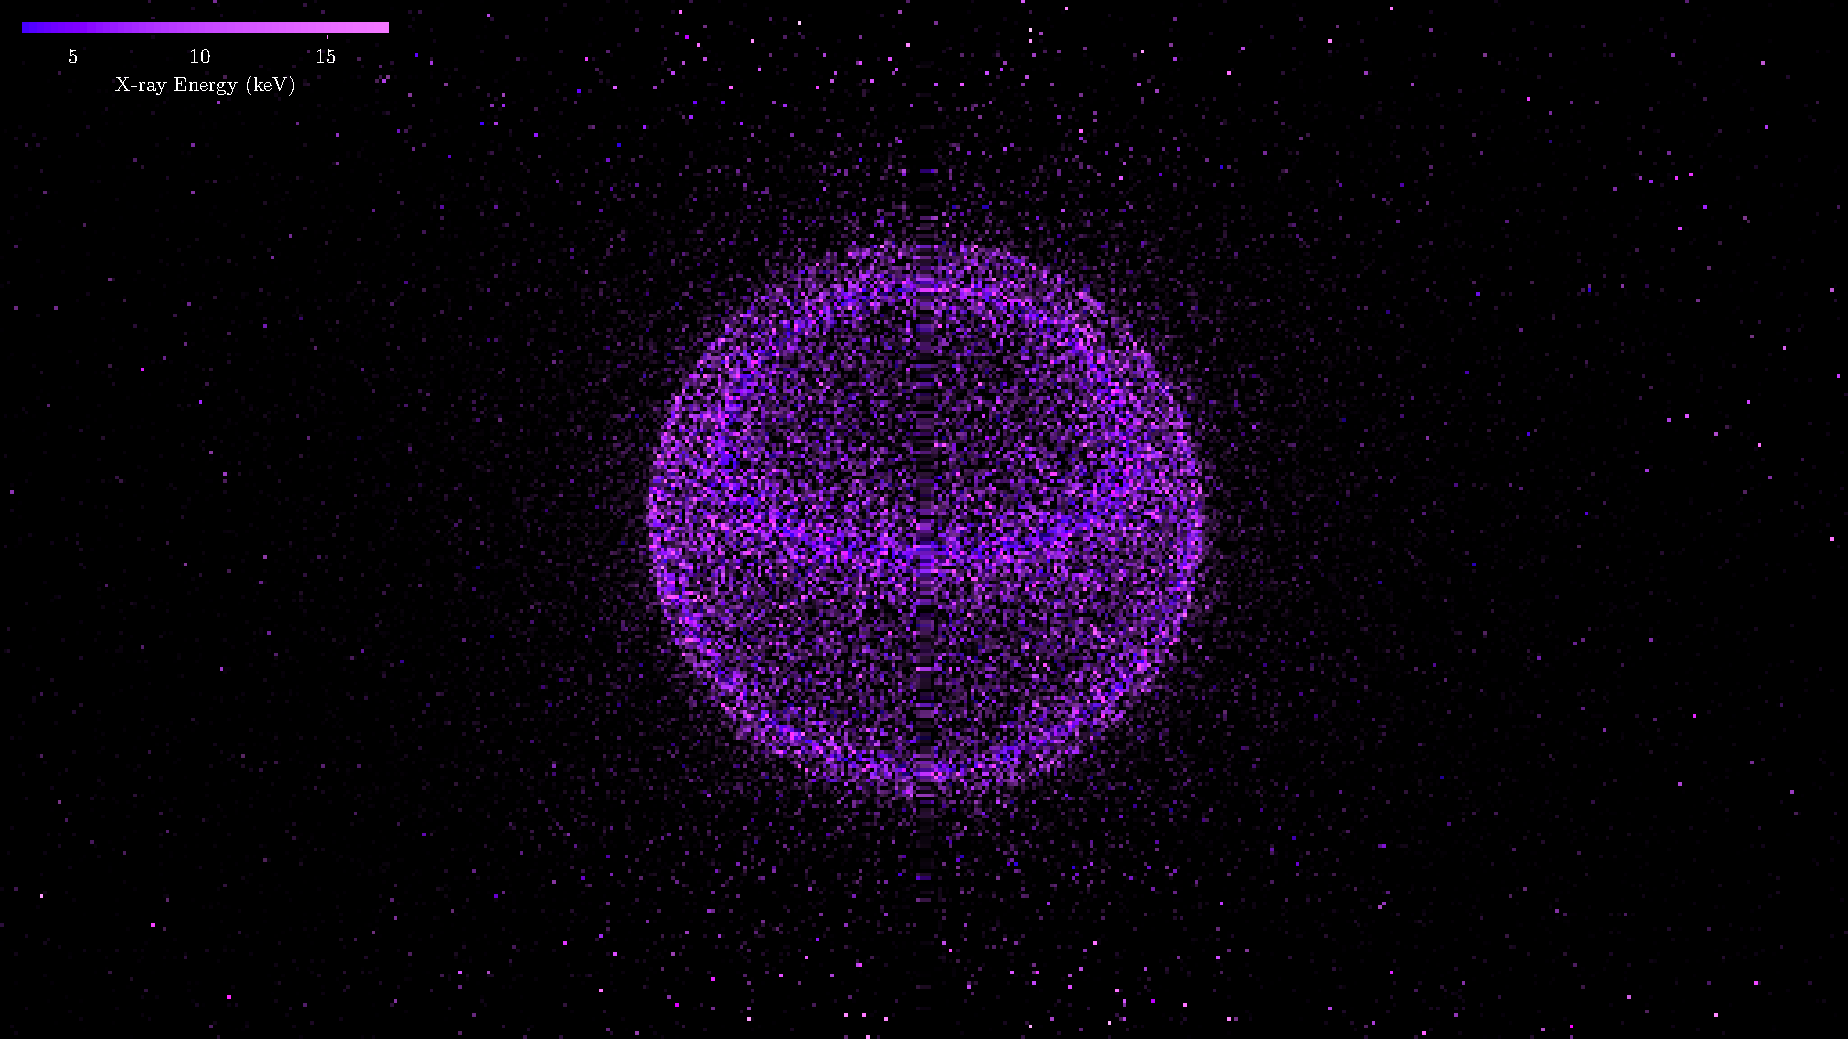
\includegraphics[width=\linewidth]{../data/schwarzschild-bright-xray.pdf}
  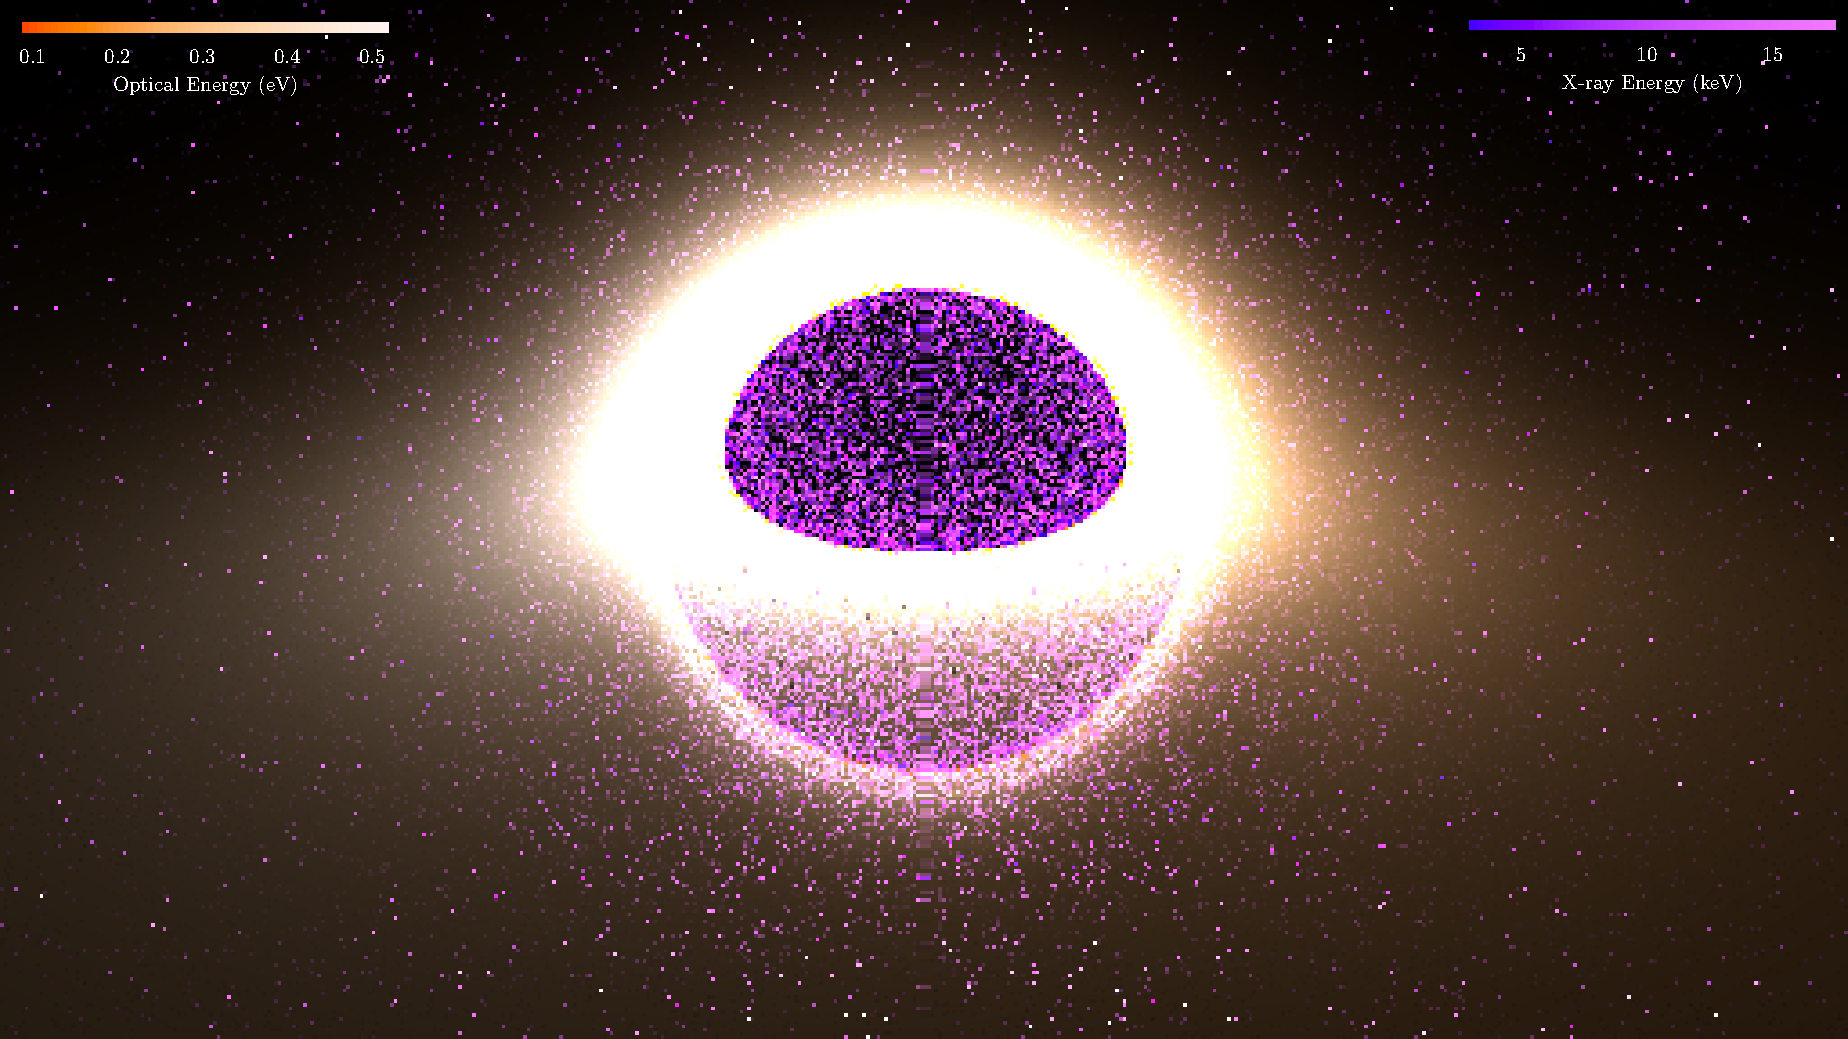
\includegraphics[width=\linewidth]{../data/schwarzschild-tog.pdf}
  \caption{(\textit{Top}) The Schwarzschild geometry in the X-ray band, which contains only IC scattered light. Near-horizon emission is much stronger than in the visible case. (\textit{Bottom}) A composite image showing both X-ray and visible light.}
  \label{fig:sch}
\end{figure}


\begin{figure}
  \centering
  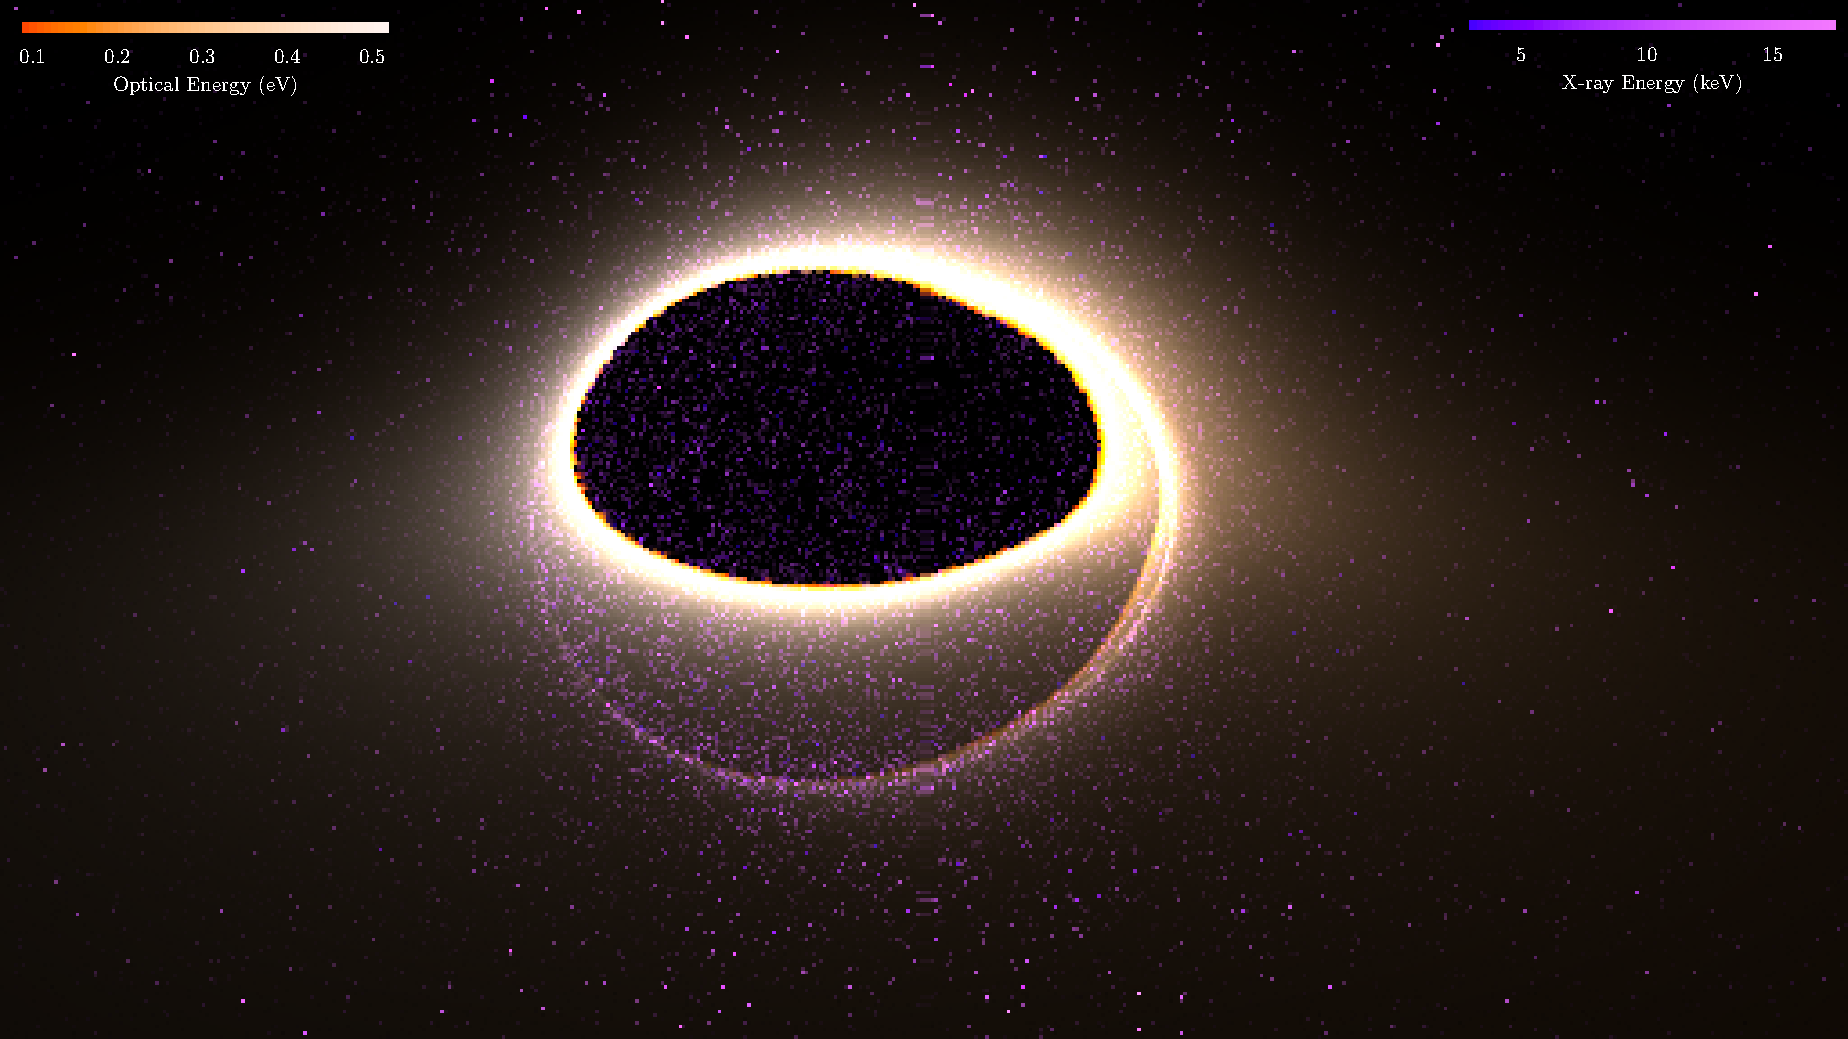
\includegraphics[width=\linewidth]{../data/kerr-tog.pdf}
  \caption{Visible and X-ray emission in the Kerr geometry with $a = 0.8$. The egg shape of the disk is a result of the BH twisting photon geodesics.}
  \label{fig:kerr}
\end{figure}

All images so far have not displayed a BH corona, but figure \ref{fig:sch} models the corona and depicts the corresponding X-ray flux. By assumption that the corona density $\rho_0$ is small enough that IC scattering is unlikely, the visible flux of the BH is mostly unchanged. The top panel of the figure however depicts an appreciable population of X-rays emanating from all points near the black hole, even regions where visible light cannot emanate. This is due to the ability of IC scattering to change the photon direction. IC scattering is also much closer to the BH than disk scattering, falling off sharply outside the photon ring. This is due to the higher density of the corona near the EH, and the fact that electrons inside the photon ring spend more time in that region. The ring itself is slightly visible, though not as clearly as in the visible case. This is partly due to the lack of numerical precision. Faint blue lines representing redshift are also visible in the same regions where the optical light was gravitationally redshifted, showing the effects of GR on both populations of photons.

The bottom panel of figure \ref{fig:sch} presents the X-ray counts overlayed on the visible light observed from the BH. This image further highlights the fact that some regions of the image emit only in the X-ray, including the EH above and below from the disk and the space above the accretion disk. This may be interesting from an observational perspective because it means that the properties of the emission are sensitive to different regions of the system depending on their wavelength.
    
We end the discussion of this simple model by presenting the full system for the Kerr spacetime in figure \ref{fig:kerr}. The results are qualitatively similar to figure \ref{fig:sch}, though the effect of spin on the shape of the horizon can be seen, stretching it towards the blue-shifted part of the disk. This stretch disrupts the photon ring, which is no longer circular except around the equator, and causes IC emission to be slightly brighter on the blue-shifted side of the BH. Overall, the amount of IC scattering is less, even though X-ray photons are still dominant over optical photons in the upper half of the EH.

\section{Conclusion}

A simple physical model of the environment around a supermassive BH was developed and images of the lensed accretion disk generated for an M87-like system, both in the visible and X-ray bands. Several key qualitative features were observed, such as the amplification of the accretion disk behind the BH due to lensing, the importance of optical depth in the visibility of the lower half of the BH and the photon ring, the small effect of gravitational redshift on both optical and X-ray emission, the differences in optical and X-ray spatial-distribution, and the effect of BH spin on these phenomena. Ray-tracing models more complicated than this one can be further used to generate quantitative predictions for observables of a specific source, or even as a forward model to interpret observations of a BH accretion disk.

\bibliography{bib}{}
\bibliographystyle{aasjournal}

\appendix 

\section{Corona density distribution}
\label{app:corona-density}
Assuming Newtonian gravity, the differential force due to pressure on a chunk of matter with volume $dV = r^2 d\Omega dr$ and mass $\rho dV$ is $dP r^2 d\Omega$, and the force due to gravity is $-GM\rho dV / r^2$. The ideal gas law provides $P = \frac{\rho}{m_p}kT$, where we use the proton mass because electrons are comparatively so small. Equilibrium therefore requires
\begin{equation}
  \frac{d\rho}{dr} = -\frac{GM\rho}{r^2}\frac{m_p}{kT}
\end{equation}
assuming that temperature is constant throughout the cloud. The solution is
\begin{equation}
  \rho(r) = \rho_0 \exp \brackets{\frac{GMm_p}{kT}\parens{\frac{1}{r}-\text{const}}}.
  \label{eqn:intermediate-density}
\end{equation}
The kinetic energy per protons is $(\gamma_p-1) m_p c^2$ but also $\frac{9}{2}kT$ by equipartition arguments, since the non-relativistic proton has energy $\frac{3}{2}kT$ and the relativistic electron has energy $3kT$. Since $r_S = 2GM/c^2$, equation \ref{eqn:intermediate-density} can be written as (rescaling $\rho_0$)
\begin{equation}
  \rho(r) = \rho_0 \exp \parens{\frac{9r_s}{4(\gamma_p-1) r}}.
  \label{eqn:density-distro-full}
\end{equation}

This equation becomes extremely large near $r_s \approx r$, but in this region, relativistic effects dominate, making this derivation invalid. Specifically, gravity would dominate over pressure and consume matter near the EH. Taking this effect to the extreme, a corona with no pressure near the EH would show density distribution $\rho(r) \propto \frac{1}{r^2}$ for a constant flow of matter into the BH.

To approximately wed the distant behavior of equation \ref{eqn:density-distro-full} to the near-BH $1/r^2$ in-fall, we Taylor expand the exponential of equation \ref{eqn:density-distro-full} and remove the terms of order $1/r^n$ for $n\geq 3$. This yields the density distribution given in the main text.


% If the BH consumes corona matter at small $r$, other sources must supply electrons from large $r$ and the entire corona move radially inwards to transport the electrons. Conserving the mass in each region of space requires that this velocity $\beta(r)$ satisfy
% \begin{equation}
%   (d\Omega (r+dr)^2 dr)(\rho(r)+d\rho)(\beta(r) + d\beta) = d\Omega r^2 dr \beta(r),
% \end{equation}
% which corresponds to the differential equation
% \begin{equation}
%   r\rho(r)\frac{d\beta}{dr} +  r\frac{d\rho}{dr}\beta(r) +  2\rho(r)\beta(r) = 0.
% \end{equation}
% Solving this differential equation with $\beta=c$ at $r=r_s$, we get
% \begin{equation}
%   \beta(r) = e^{1/\gamma}\parens{\frac{r_S}{r}}^2\parens{\frac{\rho_0}{\rho}},
% \end{equation}


\end{document}